\chapter{Sviluppo in multipoli}

Nel capitolo precedente abbiamo risolto l'equazione di Laplace in coordinate sferiche \emph{in presenza di simmetria azimutale}, il problema del potenziale generico, tuttavia, può avere una dipendenza dalla coordinate $\varphi$, quindi adesso riportiamo una soluzione generale.

\section{Armoniche sferiche}

In caso di dipendenza azimutale, per risolvere il problema della separazione delle variabili, dobbiamo andare a trovare una soluzione per l'equazione di Legendre generalizzata (\ref{eq:Legrendre_gen}), ovvero una forma generalizzata della \ref{eq:Rodrigues}.\\

Si può dimostrare allo stesso modo visto per le funzioni di Legendre ordinarie che, affinché la \ref{eq:Legrendre_gen} ammetta soluzioni finite nell'intervallo $-1 \leq x \leq 1$, il parametro \emph{$l$ deve essere zero o un intero positivo e l'intero $m$ può assumere solo i valori $-l, -(l-1), ..., 0, ..., (l-1), l$}. La soluzione che possiede questa proprietà è \mkeyword{funzione di Legendre associata} chiamata funzione di Legendre associata $P_l ^m (x)$.\\

Per $m$ positivo, essa è definita dalla formula 

\begin{equation}
    P_l ^m (x) = (-1)^m (1 - x^2)^{m/2} \frac{d^m}{dx^m} P_l(x)
\end{equation}

Se si usa la formula di Rodrigues si ottiene una formula valida sia per $m$ positivi che negativi:

\begin{tcolorbox}[colback=yellow!10!white, colframe=orange!70!black, boxrule=0.8pt]
\begin{equation}
    P_l^m (x) = \frac{(-1)^m}{2^l l!} (1 - x^2)^{m/2} \frac{d^{l + m}}{dx^{l + m}} (x^2 - 1)^l
\end{equation}
\end{tcolorbox}

Un fatto importante è che, per $m$ fissato, le funzioni $P_l^m$ formano un insieme ortogonale nell'indice $l$ sull'intervallo $-1 \leq x \leq 1$. La relazione di ortogonalità è espressa come 

\begin{tcolorbox}[colback=yellow!10!white, colframe=orange!70!black, boxrule=0.8pt]
\begin{equation}
    \int_{-1} ^1 P_{l'}^m (x) P_l ^m (x) \ dx = \frac{2}{2l +1} \frac{(l+m)!}{(l-m)!} \delta_{l'l}
\end{equation}
\end{tcolorbox}

In questo modo la soluzione dell'equazione di Laplace è stata decomposta in un prodotto di fattori per le tre variabili $r, \theta, \varphi$. \\

\newpage

\' E conveniente combinare i fattori \mkeyword{armoniche sferiche} angolari e costruire funzioni ortonormali sulla sfera unitaria. Chiameremo queste funzioni armoniche sferiche. \\

Le funzioni \(Q_m(\varphi) = e^{im\varphi}\) formano un insieme completo di funzioni ortogonali nell’indice \(m\) sull’intervallo \(0 \le \varphi \le 2\pi\). \\
Le funzioni \(P_l^m(\cos\theta)\) formano un simile insieme nell’indice \(l\) per ogni valore di \(m\) sull’intervallo \(-1 \le \cos\theta \le 1\). \\

Il loro prodotto \(P_l^m Q_m\) formerà pertanto un insieme completo di funzioni ortogonali sulla superficie della sfera unitaria negli indici \(l, m\). 
Dalla condizione di normalizzazione è chiaro che le funzioni opportunamente normalizzate, indicate con \(Y_{lm}(\theta,\varphi)\), sono

\begin{tcolorbox}[colback=yellow!10!white, colframe=orange!70!black, boxrule=0.8pt]
\begin{equation}
Y_{lm}(\theta,\varphi)
= \sqrt{\frac{2l+1}{4\pi} \frac{(l-m)!}{(l+m)!}}\, P_l^m(\cos\theta)\, e^{im\varphi}
\end{equation}
\end{tcolorbox}

Inoltre vale che 

\begin{equation}
    Y_{l,-m}(\theta, \varphi) = (-1)^m Y_{lm}^* (\theta, \varphi)
\end{equation}

Si riportano le prime funzioni armoniche sferiche 

\begin{equation}
\begin{aligned}
l=0 \quad & \quad Y_{00} = \frac{1}{\sqrt{4\pi}} \\[6pt]
l=1 \quad &
\left\{
\begin{aligned}
Y_{11} &= -\sqrt{\frac{3}{8\pi}}\,\sin\theta\, e^{i\phi} \\
Y_{10} &=  \sqrt{\frac{3}{4\pi}}\,\cos\theta \\
\end{aligned}
\right. \\[10pt]
l=2 \quad &
\left\{
\begin{aligned}
Y_{22} &= \frac14 \sqrt{\frac{15}{2\pi}}\,\sin^{2}\theta\, e^{2i\phi} \\
Y_{21} &= -\sqrt{\frac{15}{8\pi}}\,\sin\theta\cos\theta\, e^{i\phi} \\
Y_{20} &=  \sqrt{\frac{5}{4\pi}} \left( \frac{3}{2}\cos^{2}\theta - \frac12 \right)
\end{aligned}
\right. \\[10pt]
\end{aligned}
\end{equation}

Quindi possiamo andare ad esprimere la soluzione generale del potenziale come 

\begin{tcolorbox}[colback=yellow!10!white, colframe=orange!70!black, boxrule=0.8pt]
\begin{equation}
    V(r,\theta, \varphi) = \sum_{l = 0}^{\infty} \sum_{m = -l} ^ l (A_l r^l + B_l \frac{1}{r^{l+1}}) Y_{lm} (\theta, \varphi)
\end{equation}
\end{tcolorbox}

\newpage

\subsection{Teorema di somma per le armoniche sferiche}

Un'importante espansione con i polinomi di Legendre è la seguente 

\begin{equation}
    \frac{1}{|\mathbf{x} - \mathbf{x'}|} = \sum_{l = 0}^{\infty} \frac{r_< ^l}{r_>^{l + 1}} P_l (\cos \gamma)
    \label{eq:primo_sviluppo}
\end{equation}

Dove $r_< \ (r_>)$ è il più piccolo (più grande) fra $|\mathbf{x}|$ e $|\mathbf{x'}|$ e $\gamma$ è l'angolo fra $\mathbf{x}$ e $\mathbf{x'}$.\\

Un risultato matematico di notevole interesse è noto \mkeyword{teorema di somma} come teorema di somma  per le armoniche sferiche. \\

\begin{figure} [h]
    \centering
    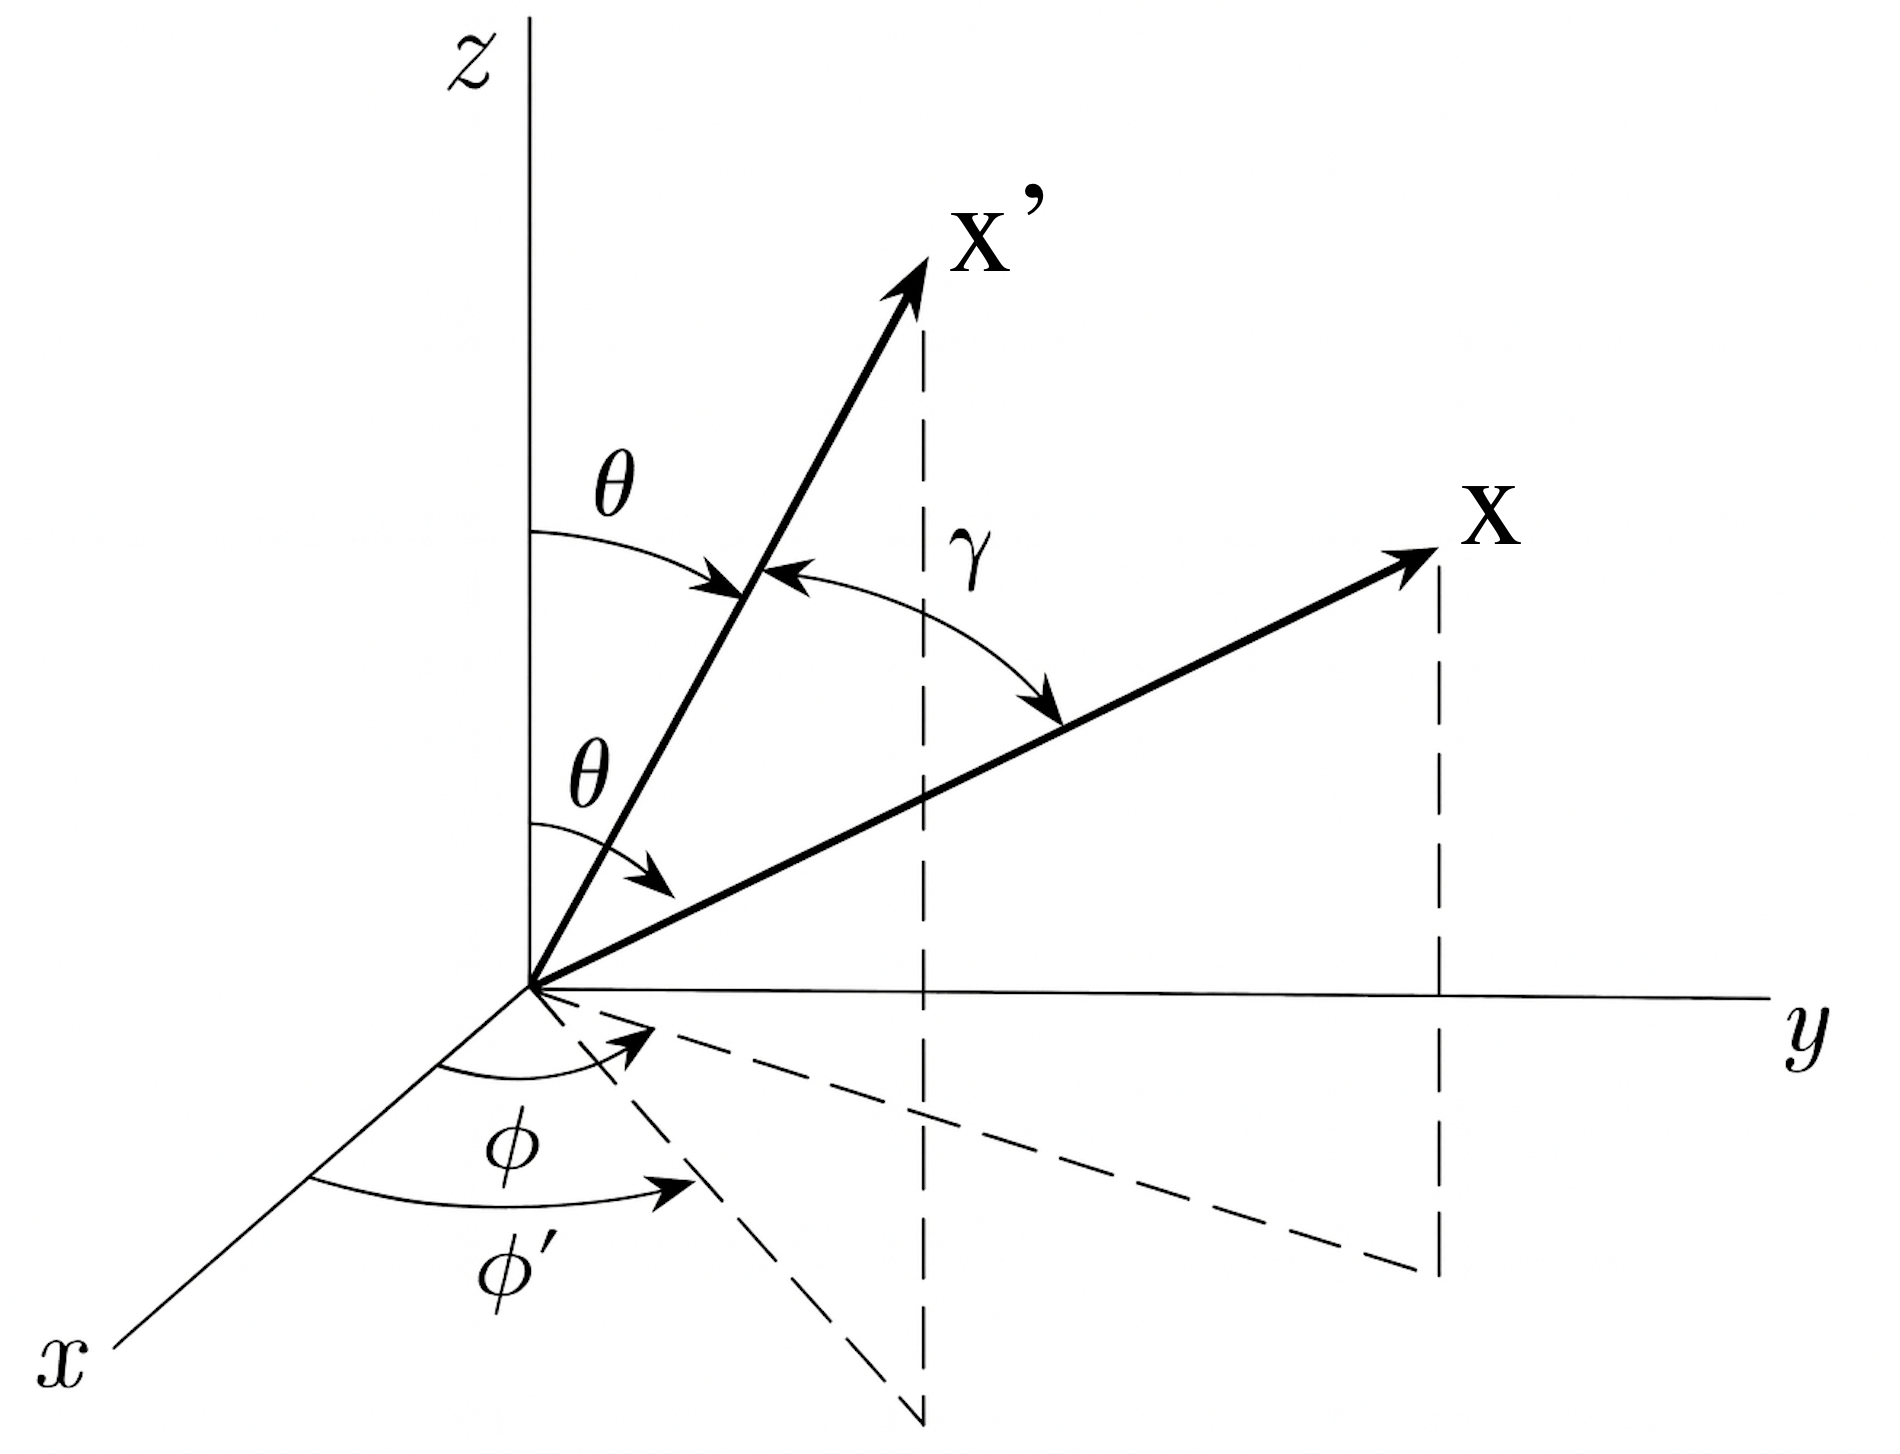
\includegraphics[width=0.5\linewidth]{figure/image29.png}
    \label{fig:chapter_10_1}
\end{figure}

Questo teorema permette di esprimere un polinomio di Legendre di ordine $l$ nell'angolo $\gamma$ in termini di armoniche sferiche negli angoli $\theta , \varphi$ e $\theta' , \varphi'$:

\begin{equation}
    P_l (\cos \gamma) = \frac{4 \pi}{2l +1} \sum_{m=-l} ^l Y_{lm}^* (\theta', \varphi') Y_{lm} (\theta, \varphi)
\end{equation}

Applicando il teorema alla \ref{eq:primo_sviluppo}, otteniamo 

\begin{tcolorbox}[colback=yellow!10!white, colframe=orange!70!black, boxrule=0.8pt]
\begin{equation}
    \frac{1}{|\mathbf{x} - \mathbf{x'}|} = 4 \pi \sum_{l=0}^{\infty} \sum_{m= -l}^{l} \frac{1}{2l +1} \frac{r_<^l}{r_>^{l+1}} Y^*_{lm} (\theta', \varphi') Y(\theta, \varphi) 
    \label{eq:espansione_rapporto_distanza}
\end{equation}
\end{tcolorbox}

\newpage

\section{Multipoli}

Supponiamo di considerare una distribuzione di carica con densità data da $\rho(\mathbf{x'})$. Il potenziale all'esterno di questa distribuzione, grazie a quanto detto prima, può essere espresso mediante uno sviluppo in armoniche sferiche 

\begin{equation}
    V(\mathbf{x}) = \frac{1}{4 \pi \varepsilon_0} \sum_{l = 0}^{\infty} \sum_{m = -l}^l  \frac{4 \pi}{2l +1} q_{lm} \frac{Y_{lm} (\theta , \varphi)}{r^{l +1}}
\end{equation}

dove la particolare scelta dei coefficienti è stata fatta per convenienza. Per risolvere il problema dobbiamo riuscire a determinare i fattori $q_{lm}$. Noi sappiamo che il potenziale di una certa distribuzione con densità $\rho(\mathbf{x})$ è esprimibile con la \ref{eq:potenziale_senza_condizione}, cioè:

\begin{equation*}
    V(\mathbf{x}) = \frac{1}{4 \pi \varepsilon_0} \int_{\tau}\frac{\rho(\mathbf{x})}{|\mathbf{x} - \mathbf{x'}|} d\tau
\end{equation*}

Ma espandendo $1/|\mathbf{x} - \mathbf{x'}|$ come \ref{eq:espansione_rapporto_distanza} otteniamo 

\begin{tcolorbox}[colback=yellow!10!white, colframe=orange!70!black, boxrule=0.8pt]
\begin{equation}
    V(\mathbf{x}) =  \frac{1}{4 \pi \varepsilon_0} \sum_{l = 0}^{\infty} \sum_{m = -l}^l  \frac{4 \pi}{2l +1} \left [ \int Y^*_{lm} (\theta',\varphi') r'^l \rho(\mathbf{x'}) d\tau \right] \frac{Y_{lm} (\theta , \varphi)}{r^{l +1}}
    \label{eq:multipolo_sferiche}
\end{equation}
\end{tcolorbox}

Da questo di capisce che 

\begin{tcolorbox}[colback=yellow!10!white, colframe=orange!70!black, boxrule=0.8pt]
\begin{equation}
    q_{lm} = \int Y^*_{lm} (\theta',\varphi') r'^l \rho(\mathbf{x'}) d\tau 
\end{equation}
\end{tcolorbox}

Questi \mkeyword{momenti di multipolo} coefficienti sono chiamati momenti di multipolo. \\

La \ref{eq:multipolo_sferiche} rappresenta il potenziale quando siamo in coordinate sferiche. In questo caso il calcolo dei momenti di multipolo è meccanico, basta risolvere l'intergrale, tuttavia da questa forma non si intuisce il significato fisico. \\
Per capire meglio il significato fisico è utile passare in coordinate cartesiane:

\begin{tcolorbox}[colback=yellow!10!white, colframe=orange!70!black, boxrule=0.8pt]
\begin{equation}
    V(\mathbf{x}) = \frac{1}{4\pi \varepsilon_0} \left[ \frac{q}{r} + \frac{\mathbf{p} \cdot \mathbf{x}}{r^3} + \frac{1}{2} \sum_{i.j} Q_{ij} \frac{x_i x_j}{r^5} +\  ...\right]
    \label{eq:multipoli_cartesiane}
\end{equation}
\end{tcolorbox}

Dove $q$ è la carica totale del sistema, $\mathbf{p}$ è il momento di dipolo di cui abbiamo parlato nei capitoli precedenti\footnote{Lo sviluppo in multipoli è particolarmente utile (se non necessario) nel caso in cui il sistema considerato sia neutro e il momento di dipolo sia nullo, proprio come anticipato nel capitolo sul dipolo elettrico.}, $Q_{ij}$ è il \mkeyword{tensore momento di quadrupolo} tensore momento di quadrupolo, mentre i puntini indicano la restante parte dello sviluppo, come l'ottupolo, l'esadecopolo etc., che abbiamo deciso di non scrivere in quanto molto lunghi e poiché nella maggior parte dei casi è sufficiente fermarsi al quadrupolo. 

\newpage

\subsection{Quadrupolo}

Vediamo come trovare il potenziale di una una distribuzione quando questa è elettricamente neutra e il momento di dipolo risulta essere nullo. \\

Se ci troviamo in questo caso allora dobbiamo sviluppare il potenziale fino al quadrupolo. Il tensore momento di quadrupolo risulta essere nella forma

\begin{tcolorbox}[colback=yellow!10!white, colframe=orange!70!black, boxrule=0.8pt]
\begin{equation} \label{eq:tensore_quadrupolo}
    Q_{ij} = \int (3x_i' x_j ' - r'^2 \delta_{ij}) \rho (\mathbf{x'}) d^3 x'
\end{equation}
\end{tcolorbox}

Dove con $i$ e $j$ si va ad indicare due delle coordinate $x,y,z$, dell'elemento che si trova in posizione $\mathbf{r'}$. \\
Allora risulta anche che ${(r')^2} = x^2 + y^2 + z^2$.  \\

Questa definizione potrebbe sembrare ancora poco chiara, per questo si riporta anche la formula del tensore momento di dipolo nel caso discreto:

\begin{equation}
    Q_{ij} = \sum_k q_k (3x_i x_j - r^2 \delta_{ij})
\end{equation}

Quindi per trovare il potenziale dobbiamo trovare il valore della matrice 

\begin{equation}
Q = 
\begin{pmatrix}
    Q_{xx} & Q_{xy} & Q_{xz} \\
    Q_{xy} & Q_{yy} & Q_{yz} \\
    Q_{xz} & Q_{yz} & Q_{zz}
\end{pmatrix}
\end{equation}

E sostituire i $Q_{ij}$ nella \ref{eq:multipoli_cartesiane}. \\

Spesso è molto utile andare ad esprimere la densità di carica come combinazione di delta di Dirac su $x,y,z$ e anche come combinazione di funzioni a scalino ($\Theta(x)$). Questo permette di sfruttare le proprietà della delta e semplificare di molto il calcolo degli integrali (che molto spesso hanno valore unitario, proprio grazie alle proprietà delle delta).\footnote{Spiegare questo argomento è più difficile di fare gli esercizi, quindi si consiglia di provare a risolvere qualche esercizio per poi rileggere questa parte di teoria}
